\chapter{Tesztelés és mérések}
\label{cha:test}

\section{A teszteléshez használt eszközök}
\label{sec:testtools}

A feldolgozólánc teszteléséhez elő kellett állítani először a komponensek futtatható változatát. A komponensek implementációjakor használt Bndtools eszköz ebben is nagy segítségemre volt, mert futtatáskor a Bndtools automatikusan előállította a telepíthető csomagokat. Az egyes komponensek könyvtári függőségeit, amelyek nem részei az alap OSGi futtató környezetnek (tipikusan ezek a harmadik féltől származó könyvtárak) magamnak kellett előállítanom szintén a Bndtools segítségével.

A fordításnál előállított JAR formátumú bundle-ök módosítás nélkül telepíthetőek valamilyen OSGi alapú rendszert futtatni képes környezetbe (bundle repository-ba). Fejlesztés során a gyorsabb tesztelhetőség miatt az Eclipse saját OSGi implementációs megoldását az Equinox-ot használtam. Egy stabil változat elkészítése után pedig, bizonyos szinten automatizáltan, szkriptek segítségével telepítettem az alkalmazást a SZTAKI Cloud-ban foglalt virtuális gépre, melyet az alkalmazás futtatására készítettem elő tesztelés céljából.

A telepítési környezetben már a könnyen kezelhető Apache Felix \cite{apachefelix} OSGi implementációját használtam, mert annak WebConsole eszközével könnyedén kezelhetőek a komponensek menedzselése, valamint parancssoros hozzáférés is lehetséges, ahol interaktív módon menedzselhetőek a komponensek, sőt még egy egyszerűbb Bash szintaktikáját utánzó szkriptelési lehetőséget is használhatnak a fejlesztők. Teszteléskor a virtuális gépre SSH-n belépve, az Apache Felix konzolos felületét használva telepítettem az elkészített bundle-öket és függőségeiket.

\begin{figure}[htp]
\centering
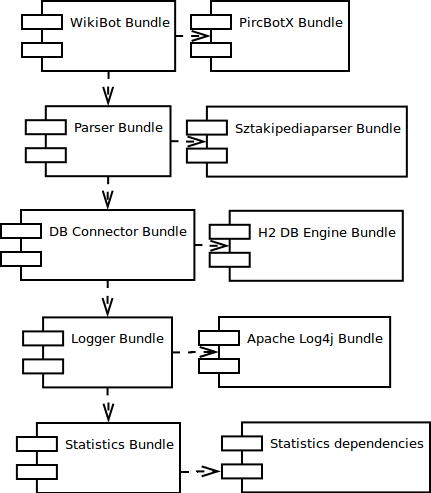
\includegraphics[scale=0.4]{img/deploymentdependency}
\caption{Komponensek függőségei}
\label{fig:deploymentdependency}
\end{figure}

Telepítéshez, illetve a feldolgozólánc komponenseinek frissítéséhez az Apache Felix egy beépített megoldását az Apache Felix Gogo-t használtam, mely egy egységes, szabványos shell felületet határoz meg az OSGi alapú környezetek számára. Amint már említettem az Apache Felix Gogo-val a Unix rendszerekben ismert Bash szintaktikához hasonló parancsokat lehet használni. Ezeket a parancsokat akár szkript formájában is futtathatjuk, ez a Gogo Shell szkript, másnéven \textit{gosh} szkript.

A csomagok függőségeit ábrázolja a \ref{fig:deploymentdependency}.~ábra. A függőségi fa leveleiben található bundle-öket kell először, majd a fában a gyökér felé visszafelé haladva kell a többi bundle-t telepíteni.

A bundle-ök menedzselését a konzolos Apache Felix Gogo Shell-en kívül, egy webes felületen Apache Felix Web Console segítségével is lehet végezni. Segítségével a rendszer állapotát, tulajdonságait lehet beállítani és megfigyelni, valamint a bundle-ök részletes tulajdonságait, kapcsolatait lehet felderíteni, illetve beállításait módosítani. A webes felületről a bundle-ök telepítésével, indításával kapcsolatos funkciók szintén elérhetőek.

% section testtools (end)

\section{A feldolgozóláncra épülő kutatómodul}
\label{sec:researchbundle}

A tesztelés során egy lehetséges felhasználási módot próbáltam ki, mikor a feldolgozólánchoz egy MTA SZTAKI által készített kutatómodult illesztettem. A modul segítségével gépi tanulás, természetes nyelvi feldolgozás témakörökhöz használható program készíthető.

A kutatómodul a feldolgozólánc által készített adatbázisból szerzi meg a bemenő adatokat, ehhez a DB Connector komponens kiegészítése volt szükséges, az OSGi szolgáltatást a lekérdezésekhez szükséges metódussal kellett ellátni. A lekérdezett cikk szövegét, melyet a Parsoid parser HTML / RDFa formátumra alakított, először szintaktikailag helyes XML formátumba kell hozni (valid XHTML).

A kutatómodul a Wikipedia eltárolt cikkeiből ún. AnnotatedDocument példányokat tud készíteni, melyekben a különböző HTML elemek kategóriák szerint vannak már csoportosítva (például: linkek, paragrafusok). Az elkészített gyűjtemények alapján OpenNLP segítségével olyan természetes nyelvi feldolgozáshoz kapcsolódó feladatok végezhetőek, mint például a mondatokra bontás, szóelemzés, tokenizálás.

A kutatómodul végső felhasználása lehet például egy adott kifejezés hivatkozásainak összegyűjtése, hogy milyen kontextusban fordulnak elő a leggyakrabban, meghatározható egy nyelv átlagos szava, vagy bekezdése, rengeteg lehetőség elképzelhető.

% section researchbundle (end)

\section{Mérési eredmények}
\label{sec:measurement}

% TODO

% section measurement (end)

% chapter test (end)